\subsection{Grundlagen des Protokolls}

Für ein Peer-to-Peer Netzwerk gibt es verschiedene Typen. Abbildung \ref{p2p_typen} zeigt 
vier Typen und ihre Unterteilung in unstrukturierte und strukturierte Netzwerke.

\begin{center}
    \captionsetup{type=figure}
    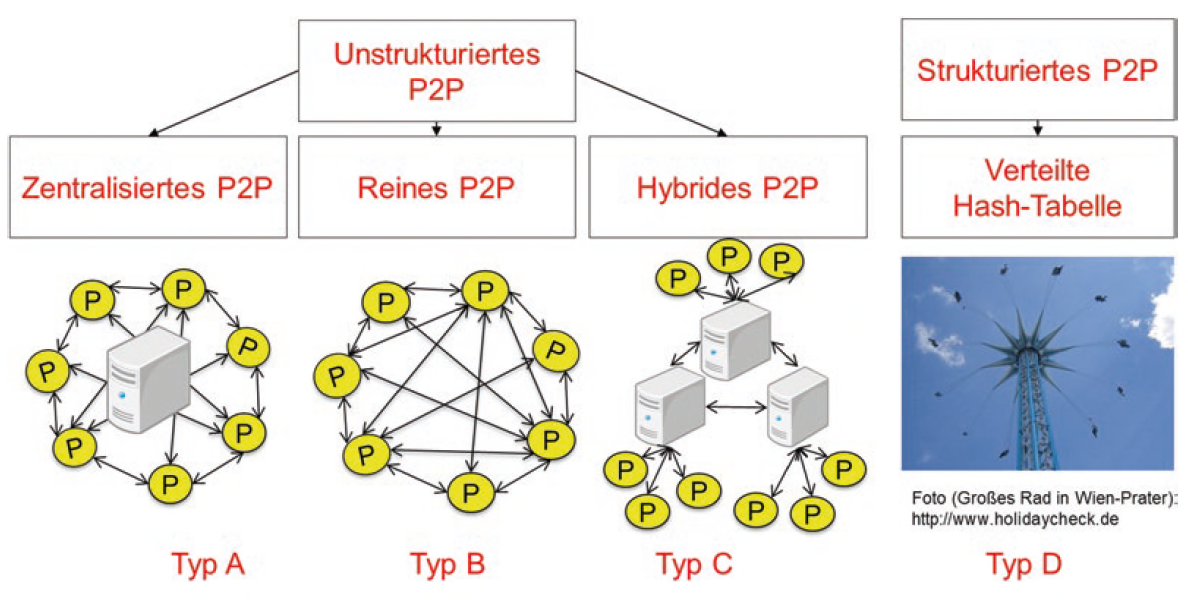
\includegraphics[width=1\linewidth]{images/peer_to_peer_typen.png}
    \captionof{figure}{Typen von Peer-to-Peer Netzwerken \parencite{Luntovskyy_ModRechnernetze}}
    \label{p2p_typen}
\end{center}

\noindent Das Protokoll dieser Arbeit fällt in die Kategorie der hybriden Peer-to-Peer Netzwerke.
Es ist sowohl strukturiert als auch unstrukturiert. Alle Teilnehmer sind in einem Netzwerk organisiert,
das aus verschiedenen Knoten besteht, wobei jeder Knoten einen Teilnehmer des Netzwerks repräsentiert.
Alle Knoten im Netzwerk sind untereinander verbunden und können Textnachrichten direkt, ohne die Verwendung 
eines Servers austauschen. Sollte sich jedoch der gewünschte Empfänger nicht im Netzwerk befinden, besteht
die Möglichkeit, dass sich der Empfänger hinter einem NAT-Gateway oder einer Firewall befindet. In diesem
Fall wird die Nachricht über einen Server, genauer gesagt über ein TCP-Relay, an den Empfänger weitergeleitet.
Der Server ist nur für die Weiterleitung der Nachricht zuständig und speichert diese nicht. Dies ist
ein Unterschied zu anderen Instant-Messaging-Protokollen, wie zum Beispiel \textcolor{red}{[Beispiel 
finden oder Satz weglassen]}, bei dem der Server die Nachrichten speichert, wenn der Empfänger offline ist. 
Das Protokoll dieser Arbeit ist also ein hybrides Peer-to-Peer-Protokoll, da es sowohl strukturierte 
als auch unstrukturierte Eigenschaften aufweist.

